% Provenance (never printed): see sources/outline_sources.md (Year 2: ore deposits ---
% magmatic, hydrothermal, sedimentary and supergene deposits; grade and tonnage; exploration).
% Deposit descriptions from the USGS Mineral Deposit Models for Resource Assessment
% (Scientific Investigations Report 2010-5070, chapters A, B, C, E, I, L, N, O, Q), USGS
% Open-File Report 03-077 (orogenic gold) and Grabreck et al. 2022 (kimberlites); the grade and
% tonnage data of the world's porphyry copper deposits from USGS Open-File Report 2008-1155
% (dataset bachelor-2-porphyry-cu). Ledger rows in sources/ledger/book4.md; curves and numbers
% from figdata/bachelor-2/ores.py and the Book 4 second-writer scratch calculator calc/ch29.py.
% Geology and sourced numbers only: no advocacy.
\chapter{مكامن الخامات}\label{ch:b2:ore-deposits}

يشكّل النحاس نحو \qty{0.006}{\percent} من القشرة؛ ويُستخرج من صخر يحتوي على نحو
\qty{0.5}{\percent}. فكلّ منجم نحاس يقع إذن على صخر أغنى بنحو ثمانين مرّة من
القشرة المحيطة به، وكلّ \omterm{def:b2:ore-deposits:deposit}{مكمن خام} هو من صنع مركِّز طبيعي: صهارة
انفصل عنها سائل كبريتيدي، أو محلول ملحي ساخن أذاب الفلزات ثم أرساها في كسر، أو
نهر فرز الحبيبات الثقيلة عن الخفيفة، أو مطر غسل الجزء العلوي من جسم خام وأعاد
ترسيب نحاسه في الأسفل. ويتتبّع هذا الفصل هذه المركِّزات، ثم يقيس
نواتجها --- كم من الخام، وبأيّ عيار --- ويختم بالطريقة التي تُكتشف بها المكامن.
% ledger: perkins:ore-grades

\begin{recall}
\textbf{من مجلّدات المدرسة}: \omterm{def:b2:ore-deposits:deposit}{مكمن الخام} \omterm{def:b2:ore-deposits:cf}{ومعامل التركيز}، والعرق المعدني، \omterm{def:b2:ore-deposits:placer}{والرواسب اللحقية}، والاحتياطي
والمورد؛ والدوران الحرمائي والمداخن السوداء عند الظهرات. \textbf{من كتب
الكيمياء}: الخام؛ والذوبانية، والأيونات المعقّدة والأكسدة والاختزال. \textbf{من مجلّد السنة الأولى}: سرعة
ترسّب الحبيبة وقانون ستوكس؛ واللاتريت؛ والرسوب التبخّري. \textbf{من
\cref{ch:b2:elements-in-the-earth}}: \omterm{def:b2:elements-in-the-earth:goldschmidt}{العنصر المحبّ للكبريتيد}، \omterm{def:b2:elements-in-the-earth:partition}{ومعامل التوزيع بين المعدن
والمصهور}. \textbf{من \cref{ch:b2:magmatic-differentiation}}: \omterm{def:b2:magmatic-differentiation:cumulate}{المتداخل الطبقي}
\omterm{def:b2:magmatic-differentiation:cumulate}{والمتراكم}. \textbf{من \cref{ch:b2:precambrian-earth}}: \omterm{def:b2:precambrian-earth:bif}{تكوين الحديد الشريطي}، \omterm{def:b2:precambrian-earth:craton}{والكراتون}.
\textbf{من كتب الرياضيات}: التوزيعان الطبيعي واللوغاريتمي الطبيعي، ودالّة التوزيع
الطبيعي $\Phi$.
\end{recall}

\section{الخام والعيار والتركيز}\label{sec:b2:ore-deposits:grade}

\begin{definition}[الشوائب]\label{def:b2:ore-deposits:ore}
\emph{الشوائب}\index{الشوائب} في الخام هي كلّ ما لا قيمة اقتصادية له: المعادن
المكوِّنة للصخر، والمعادن الحرمائية ومعادن التجوية التي ترافق معادن الخام وتُفصل
عنها وتُطرح أثناء المعالجة.
\end{definition}

ومعظم الخام شوائب. ففي \omterm{def:b2:ore-deposits:hydrothermal}{مكمن النحاس البورفيري}، المصدر الرئيسي للنحاس في العالم، تشكّل \omterm{def:b2:ore-deposits:ore}{الشوائب} أكثر من
\qty{98}{\percent} من الخام، وتشكّل معادن النحاس الباقي.
% ledger: usgs10b:share

\begin{definition}[عيار الخام، عيار القطع، الكتلة الطنّية]\label{def:b2:ore-deposits:grade}
\emph{عيار الخام}\index{عيار الخام} لحجم من الصخر هو الكسر الكتلي للعنصر
أو المعدن الثمين فيه: بالنسبة المئوية للفلزات الأساسية، وبالغرامات في الطنّ للذهب والفضّة
وعناصر مجموعة البلاتين. و\emph{عيار القطع}\index{عيار القطع} هو أدنى عيار
تُعدّ عنده كتلة من الصخر خامًا؛ وما دونه تكون الكتلة نفاية.
و\emph{الكتلة الطنّية}\index{الكتلة الطنّية} لمكمن هي كتلة الصخر الذي يفوق عياره عيار القطع؛ ومع
عيارها المتوسّط $\bar g$ تعطي الفلز المحتوى، $M = T\bar g$.
\end{definition}

\omterm{def:b2:ore-deposits:grade}{فالكتلة الطنّية} لمكمن وعياره ليسا إذن حقيقتين عن الصخر، بل جوابين
عن سؤال واحد يُطرح عند عيار قطع معيّن. فمكمن باتو هيجاو، وهو مكمن نحاس وذهب بورفيري في
إندونيسيا، يُعلَن بكتلة \qty{914}{Mt} وعيار \qty{0.53}{\percent} من النحاس فوق عيار قطع
\qty{0.3}{\percent}، وبكتلة \qty{1640}{Mt} وعيار \qty{0.44}{\percent} في تجميع عالمي
يأخذ أدنى عيار قطع متاح: فخفض \omterm{def:b2:ore-deposits:grade}{عيار القطع} يكاد يضاعف \omterm{def:b2:ore-deposits:grade}{الكتلة الطنّية}
ويخفض العيار المتوسّط. وفي مكمن زنك ورصاص رسوبي، هو مكمن توم في كندا، من شأن خفض
\omterm{def:b2:ore-deposits:grade}{عيار القطع} بنحو واحد في المئة من الزنك والرصاص معًا أن يضاعف الاحتياطيات خمس مرّات.
% ledger: usgs10b:cutoffs, usgs08:tonnage-def, usgs10n:sedex

\begin{definition}[معامل التركيز]\label{def:b2:ore-deposits:cf}
\emph{معامل التركيز}\index{معامل تركيز} لعنصر في خام هو النسبة
$\mathrm{CF} = g/a$ بين عياره $g$ ووفرته $a$ في خزّان مرجعي يُذكر معه:
القشرة القارّية كلّها، أو القشرة القارّية العليا، أو الصخر الذي تكوّن منه المكمن.
\end{definition}

ويتوقّف المعامل على المرجع. فإذا أخذنا \qty{0.006}{\percent} من النحاس للقشرة
و\qty{0.5}{\percent} للخام كان المعامل 83؛ وإذا أخذنا القشرة القارّية العليا،
\qty{28}{ppm}، ومتوسّط عيار النحاس البورفيري لعام 2008، \qty{0.44}{\percent}، كان 157. أمّا الذهب،
بمقدار \qty{1.5}{ng/g} في القشرة العليا، والمستخرج بعيار بضعة غرامات في الطنّ، فمعاملاته
بالآلاف؛ والحديد، بنسبة عدّة في المئة في القشرة، والمستخرج بعيار نحو \qty{50}{\percent}، لا يحتاج
إلا إلى معامل يقارب العشرة.
% ledger: perkins:ore-grades, rg03:ucc-trace, usgs10b:share, earle:ore-grades, earle:iron-grade

\begin{definition}[مكمن الخام]\label{def:b2:ore-deposits:deposit}
\emph{مكمن الخام}\index{مكمن خام} كتلة من الصخر ركّزت فيها عمليات طبيعية
عنصرًا أو معدنًا بعيار يفوق \omterm{def:b2:ore-deposits:grade}{عيار القطع}، وبكتلة طنّية كبيرة بما يكفي
لاستخراجه بربح. وهو في آن واحد شيء جيولوجي، تحدّده العمليات التي
كوّنته، وشيء اقتصادي، تحدّده الأسعار والتكاليف والتقنية.
\end{definition}

وبسبب نصفه الاقتصادي، يتغيّر حجم المكمن مع الزمن. فالموارد المحدَّدة
لعنصر ما هي التركيزات التي يكون استخراجها ممكنًا الآن أو قد يصبح كذلك؛ واحتياطياته
هي الجزء الذي كان يمكن استخراجه اقتصاديًا عند تحديدها. وكانت احتياطيات النحاس العالمية
\qty{280}{Mt} عام 1970؛ واستُخرج منذ ذلك الحين نحو \qty{697}{Mt}، ومع ذلك
بلغت \qty{980}{Mt} عام 2024.
% ledger: usgs:mcs-reserves

\begin{proposition}[الحصيلة الكتلية لمكمن]\label{prop:b2:ore-deposits:mass-balance}
مكمن يحوي كتلة $M$ من عنصر بعيار متوسّط $g$ غذّاه مصدر كانت فيه وفرة
العنصر $a$. فإذا انتزعت العملية المركِّزة كسرًا $\eta \leq 1$ من
العنصر من المصدر وأوصلته إلى المكمن، كانت كتلة صخر المصدر المعالَجة
\begin{equation}
m_{\mathrm{source}} = \frac{M}{\eta\,a} = \frac{\mathrm{CF}}{\eta}\, T ,
\label{eq:b2:ore-deposits:mass-balance}
\end{equation}
حيث $T = M/g$ \omterm{def:b2:ore-deposits:grade}{الكتلة الطنّية} و$\mathrm{CF} = g/a$: أي ما لا يقلّ عن CF طنًّا من المصدر لكلّ طنّ من الخام.
\end{proposition}

\begin{proof}
فقد المصدر $\eta\,a\,m_{\mathrm{source}}$ من العنصر وتلقّى المكمن $M$؛ ومساواة
الكمّيتين تعطي الصيغة الأولى، و$M = gT$ تعطي الثانية. وبما أنّ $\eta \leq 1$، فإنّ $m_{\mathrm{source}} \geq
\mathrm{CF}\,T$.
\end{proof}

فمكمن بينغهام كانيون، المكمن البورفيري المبيّن أدناه، مُدرج بكتلة \qty{3230}{Mt} وعيار
\qty{0.882}{\percent} من النحاس، أي \qty{28.5}{Mt} من النحاس. ومعامل تركيزه مقارنة بالقشرة العليا 315،
وحتى عملية تامّة الكفاءة كان عليها أن تستنزف \num{1.02e12} طنّ من القشرة العليا
المتوسّطة، أي نحو \qty{377}{km^3}: مكعّبًا طول ضلعه \qty{7.2}{km}. فالعمليات المكوِّنة للخامات
هي إذن عمليات تنقل كثيرًا من المادّة --- صهارة، وماء، ورواسب --- عبر حجم
صغير يُحتجز فيه العنصر.
% ledger: data:b4-porphyry-cu, rg03:ucc-trace
% values: 28.49 Mt; CF 315; 1.0175e12 t; 377 km3 at 2.7 t/m3; side 7.22 km (calc/ch29.py)

\begin{omfigure}
\centering
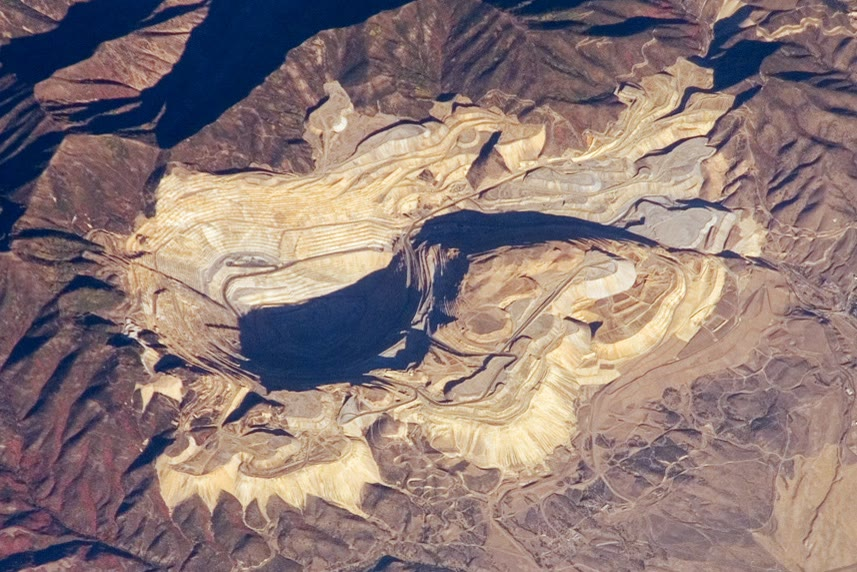
\includegraphics[width=0.5\linewidth]{images/book4/b2-29-bingham-canyon-iss.jpg}
\par\smallskip{\small حفرة بينغهام كانيون المكشوفة، يوتا، من محطّة الفضاء الدولية
(2007): يزيد عرضها على \qty{4}{km} وعمقها \qty{1200}{m}، وقد حُفرت بمصاطب ارتفاعها من 16 إلى \qty{25}{m}
في مكمن نحاس بورفيري؛ والتلال المسطّحة القمم حولها هي صخور النفاية. الصورة:
ناسا، طاقم البعثة 15 (ملك عام).}
\end{omfigure}
% ledger: photo:b2-29-bingham

\begin{definition}[أنماط مكامن الخام]\label{def:b2:ore-deposits:types}
\emph{نمط مكامن الخام}\index{نمط مكامن الخام} صنف من المكامن تشترك في الإطار
الجيولوجي، والصخر المضيف، والشكل، ومعدنية الخام وعملية التكوّن، بحيث يتنبّأ وصف
الصنف بالأماكن التي يوجد فيها أفراده. وتنقسم الأنماط إلى أربع عائلات بحسب العملية:
الصهارية (تركّز الفلزَّ صهارةٌ وهي تتبلور أو تنفصل إلى سائلين غير ممتزجين)،
والحرمائية (يركّزه مائع مائي ساخن)، والرسوبية (بنقل الرواسب وترسيبها،
أو بالترسّب الكيميائي من الماء عند السطح)، والسوبرجينية (بتجوية
مكمن سابق).
\end{definition}

\section{المكامن الصهارية}\label{sec:b2:ore-deposits:magmatic}

\textbf{الكروميت في المتداخلات الطبقية.} الكروميت، المصدر التجاري الوحيد للكروم،
يتجمّع في طبقات من الكروميتيت الكتلي، الذي يزيد محتواه من الكروميت على \qty{90}{\percent}، في الأجزاء
السفلى فوق المافية من المتداخلات الطبقية. ويتراوح عرض هذه المتداخلات بين 2 و\qty{180}{km} ويصل سمكها إلى
\qty{15}{km}، ويتراوح سمك الطبقات من أقلّ من سنتيمتر إلى 5--\qty{8}{m}؛ وهي تحوي معًا
معظم احتياطيات الكروم في العالم، ومعقّد بوشفيلد، الذي مرّ في
\cref{ch:b2:magmatic-differentiation}، هو الوحيد الذي يُستخرج منه الكروميت اليوم. وأصلها،
طبقة متراكمة دُفعت إلى حقل استقرار الكروميت بفعل اختلاط الصهارات أو تغيّر الضغط أو
حالة الأكسدة، لا يزال موضع جدل.
% ledger: usgs10e:chromite

\textbf{كبريتيدات النيكل والنحاس وعناصر مجموعة البلاتين.} صهارة مافية أو فوق مافية، ناتجة عن درجات انصهار كبيرة
للوشاح (من \qty{20}{\percent} إلى \qty{25}{\percent} أو أكثر، وأكثر من 12 في المئة وزنًا من MgO)،
تصعد غير مشبعة بالكبريت. فإذا تمثّلت كبريتًا من القشرة، أو بردت بما
يكفي، أصبحت مشبعة وانفصل عنها سائل كبريتيدي غير ممتزج في قطيرات. وتنتقل
الفلزات المحبّة للكبريتيد إلى هذه القطيرات: فالنسبة $D$ بين تركيزها في السائل
الكبريتيدي وتركيزها في السائل السيليكاتي، وهي معامل توزيع من النوع نفسه الذي بين
معدن ومصهور، تتراوح من $10^2$ إلى $10^3$ للنحاس والنيكل ومن $10^3$ إلى $10^4$ لعناصر
مجموعة البلاتين. وكمّية الفلز التي تجمعها القطيرة تتوقّف عندئذ على كمّية \omterm{def:b2:magma-emplacement:magma}{الصهارة} التي تلاقيها.
% ledger: usgs10i:r-factor

\begin{proposition}[العامل R]\label{prop:b2:ore-deposits:r-factor}
ليكن سائل كبريتيدي كتلته الوحدة ينفصل عن كتلة $R$ من \omterm{def:b2:magma-emplacement:magma}{الصهارة} السيليكاتية، ويبلغ معها التوازن،
وهي \emph{العامل R}\index{العامل R}، في نظام مغلق؛ وليكن $C_L$ تركيز
فلز في \omterm{def:b2:magma-emplacement:magma}{الصهارة} قبل انفصال الكبريتيد، و$D$ معامل توزيعه بين الكبريتيد
والسيليكات. عندئذ يكون تركيز الفلز في الكبريتيد
\begin{equation}
C_S = C_L\,\frac{D\,(R + 1)}{R + D} .
\label{eq:b2:ore-deposits:r-factor}
\end{equation}
عندما $R \gg D$ يكون $C_S \to D\,C_L$؛ وعندما $R \ll D$ يكون $C_S \approx (R + 1)\,C_L$.
\end{proposition}

\begin{proof}
كان النظام ذو الكتلة $R + 1$ يحوي $(R + 1)C_L$ من الفلز قبل الانفصال. وبعده، يحوي السيليكات
$R\,C_{\mathrm{sil}}$ والكبريتيد $C_S$، مع $C_S = D\,C_{\mathrm{sil}}$ عند التوازن.
ويعطي الانحفاظ $(R + 1)C_L = R\,C_S/D + C_S = C_S\,(R + D)/D$، ومن ثمّ
\eqref{eq:b2:ore-deposits:r-factor}. وإذا كان $R \gg D$، فإنّ $(R + 1)/(R + D) \to 1$؛ وإذا كان $R \ll D$،
فإنّ $D/(R + D) \to 1$.
\end{proof}

ويفسّر الحدّان سبب وجود نوعين من خامات الكبريتيد. فعندما $R \ll D$ يأخذ الكبريتيد
كلّ فلز \omterm{def:b2:magma-emplacement:magma}{الصهارة} التي يلاقيها تقريبًا ويزداد $C_S$ مع $R$؛ وعندما $R \gg D$ يكون
مشبعًا عند $D\,C_L$ ولا تضيف \omterm{def:b2:magma-emplacement:magma}{الصهارة} الإضافية شيئًا. فالنيكل والنحاس، وقيمة $D$ لهما بضع مئات،
يبلغان سقفهما عند $R$ من بضع مئات إلى بضعة آلاف، وهو مدى معظم خامات النيكل والنحاس؛
أمّا البلاتين والبلاديوم، وقيمة $D$ لهما قرب $10^4$، فيظلّان يكسبان حتى $R$ من \num{10000} إلى
\num{100000}. ولذلك فإنّ الخامات الغنيّة بعناصر مجموعة البلاتين، مثل حيد ميرنسكي في بوشفيلد
وبعض خامات نوريلسك، تسجّل كتلة صغيرة من الكبريتيد غسلتها كتلة كبيرة جدًا من
\omterm{def:b2:magma-emplacement:magma}{الصهارة} (التمرينان~\ref{exo:b2:ore-deposits:5} و\ref{exo:b2:ore-deposits:11}).
% ledger: usgs10i:r-factor

\textbf{الكمبرليت والألماس.} تكوّن معظم الألماس، وكلّ المستخرج منه تقريبًا، عند قاعدة
الليثوسفير القارّي السميك، في جذور الكراتونات؛ وتحمله صهارات الكمبرليت، الآتية من أعماق
تزيد على 120 إلى \qty{150}{km} والصاعدة بسرعة تصل إلى \qty{20}{m.s^{-1}}، إلى
السطح بسرعة تكفي لبقائه. وتندفع الكمبرليتات مفضّلةً عبر الليثوسفير السميك القديم،
وهناك يبحث المنقّبون عن الألماس.
% ledger: grabreck22:kimberlite

\textbf{البيغماتيت.} بيغماتيتات الليثيوم والسيزيوم والتنتالوم قواطع غرانيتية غنيّة بهذه العناصر
النادرة، تتكوّن في الأوروجينات التصادمية؛ وتتبلور عند نحو 350 إلى \qty{550}{\celsius}،
وهي حرارة منخفضة على نحو لافت لمصهور غرانيتي، في أيام إلى سنوات، وتنمو فيها بلّورات هائلة --- فقد بلغ طول
بلّورة سبودومين واحدة \qty{14}{m}. ومعادنها الليثيومية، السبودومين والبيتاليت
والليبيدوليت، تزوّد العالم بنحو ربع إنتاجه من الليثيوم.
% ledger: usgs10o:lct

\section{المكامن الحرمائية}\label{sec:b2:ore-deposits:hydrothermal}

\begin{definition}[المائع الحرمائي وأنماط المكامن الحرمائية]\label{def:b2:ore-deposits:hydrothermal}
\emph{المائع الحرمائي}\index{المائع الحرمائي} مائع مائي ساخن، تطلقه صهارة،
أو تفاعلات تحوّلية، أو ماء بحر أو ماء جوّي أو محلول ملحي حوضي سُخّن، يذيب العناصر
وينقلها ويرسّبها وهو يجري عبر الصخر. وأهمّ أنماط مكامن الخام الحرمائية
هي:
\begin{itemize}
  \item \emph{مكمن النحاس البورفيري}\index{مكمن النحاس البورفيري}: جسم كبير منخفض العيار
        من العروق الدقيقة وكبريتيدات النحاس المنتشرة في كتلة بورفيرية صغيرة وحولها، تكوّن من
        موائع صهارية على بعد بضعة كيلومترات من السطح فوق نطاق اندساس؛
  \item \emph{المكمن الإبيثرمي}\index{المكمن الإبيثرمي}: عروق ذهب وفضّة وانتشارات
        تكوّنت على عمق لا يتجاوز نحو \qty{1.5}{km} من السطح، عند نحو 100 إلى
        \qty{300}{\celsius}، في الأقواس البركانية؛
  \item \emph{مكمن الكبريتيدات الكتلية البركانية المنشأ}\index{مكمن الكبريتيدات الكتلية البركانية المنشأ}
        (VMS): عدسة من الكبريتيدات الكتلية تكوّنت على قاع البحر أو تحته مباشرة، عند فوهة
        حرمائية في بيئة بركانية تحت بحرية؛
  \item \emph{المكمن الرسوبي النفثي}\index{المكمن الرسوبي النفثي} (سيديكس):
        كبريتيدات زنك ورصاص مصفّحة في طَفل بحري لحوض صدعي، ترسّبت على قاع البحر أو
        تحته مباشرة من محاليل ملحية حوضية صاعدة على طول الصدوع؛
  \item \emph{مكمن نمط وادي المسيسيبي}\index{مكمن نمط وادي المسيسيبي} (MVT):
        كبريتيدات زنك ورصاص تحلّ محلّ كربونات المنصّات، لاحقة التكوّن ولا صلة لها بالنشاط
        الناري، رسّبتها محاليل ملحية حوضية؛
  \item \emph{مكمن الذهب الأوروجيني}\index{مكمن الذهب الأوروجيني}: عروق كوارتز حاملة للذهب في
        الأحزمة التحوّلية، على طول صدوع كبرى، رسّبتها موائع منخفضة الملوحة غنيّة بغاز CO$_2$
        ذات أصل تحوّلي.
\end{itemize}
\end{definition}
% ledger: usgs10b:form, usgs10q:epithermal, usgs10c:vms, usgs10n:sedex, usgs10a:mvt, drew03:orogenic

\textbf{النقل والترسيب.} تُحمل معظم الفلزات في الموائع الحرمائية على هيئة معقّدات:
الزنك والرصاص والنحاس على هيئة معقّدات كلوريدية، فتتحكّم الملوحة في ذوبانيتها، والذهب،
في الموائع المختزِلة، على هيئة معقّدات كبريتية مثل \babelsublr{AuHS(H$_2$S)$_3$}. ويُلقي المائع حمولته حين
تنخفض الذوبانية: حين يبرد؛ وحين يغلي مع انخفاض ضغطه، فيفقد H$_2$S وCO$_2$
ويتغيّر أسّه الهيدروجيني؛ وحين يختلط بمائع مختلف التركيب --- فالمحلول الملحي الذي يلاقي ماءً غنيًّا
بغاز H$_2$S يرسّب السفاليريت والغالينا فورًا تقريبًا؛ وحين يتفاعل مع صخر
الجدار، فيتغيّر أسّه الهيدروجيني أو حالة أكسدته. وكلّ نمط من المكامن تركيبة واحدة من المائع،
والمسار والمصيدة.
% ledger: usgs10n:sedex, drew03:orogenic

\textbf{النحاس البورفيري.} تزوّد المكامن البورفيرية العالم بنحو \qty{60}{\percent} من
نحاسه وتحوي نحو \qty{65}{\percent} من موارده. وهي تتمركز حول كتل
أسطوانية صغيرة أو حشود من القواطع، هي قمم بلوتونات أكبر، توضّعت على عمق يقلّ عن 5--\qty{10}{km}
في الأقواس فوق نطاقات الاندساس، وهي بيئة \cref{ch:b2:magmatic-series}. ويتراوح عرض المكمن بين 0.1
و\qty{1}{km}، وله ارتفاع مماثل؛ وقد يمتدّ الصخر المتبدّل \qty{10}{km} أو أكثر حوله.
ومع تبلور \omterm{def:b2:magma-emplacement:magma}{الصهارة}، ينفصل عنها مائع يحوي من 3 إلى 5 في المئة وزنًا من الملح؛ وفي صعوده
وانخفاض ضغطه، ينقسم إلى محلول ملحي وبخار، يحمل كلاهما الفلزات، ويكسّر ضغطُه الزائد
الصخر. وتترسّب عروق الكوارتز عند نحو 700 إلى \qty{500}{\celsius}، ويوزّع
تفاعل المائع مع الصخر التبدّلَ في نطاقات، كما في المقطع أدناه. ولأنّها
تتكوّن ضحلة عند الحوافّ النشطة، حيث التعرية سريعة، فإنّ أكثر من \qty{90}{\percent} من مكامن
البورفيري المعروفة تعود إلى السينوزوي أو الميزوزوي.
% ledger: usgs10b:share, usgs10b:form, usgs10b:fluids, usgs10b:alteration

\begin{omfigure}
\centering
\begin{tikzpicture}[x=1.15cm, y=1.15cm, font=\small]
\begin{scope}
\clip (-2.9,-3.6) rectangle (2.9,0);
% propylitic halo
\fill[omLithBasalt!45] (0,-1.25) ellipse (2.45 and 1.55);
% sodic-calcic deep flanks
\fill[omExo!25] (-1.75,-2.55) ellipse (0.45 and 0.38);
\fill[omExo!25] (1.75,-2.55) ellipse (0.45 and 0.38);
% sericitic shell
\fill[yellow!35] (0,-1.05) ellipse (1.15 and 1.15);
% potassic core
\fill[omProp!40] (0,-1.45) ellipse (0.68 and 0.85);
% ore shell
\draw[omThm, line width=1.1pt, densely dashed] (0,-1.3) ellipse (0.92 and 0.98);
% advanced argillic lithocap
\fill[omDef!30] (-1.05,0) .. controls (-0.6,-0.5) and (0.6,-0.5) .. (1.05,0) -- cycle;
\draw[omDef!70] (-1.05,0) .. controls (-0.6,-0.5) and (0.6,-0.5) .. (1.05,0);
\end{scope}
% pluton and stock
\fill[omLithGranite] (-2.6,-3.6) .. controls (-2.2,-2.9) and (-0.9,-2.6) .. (-0.3,-2.6)
  -- (-0.3,-1.25) arc[start angle=180, end angle=0, radius=0.3] -- (0.3,-2.6)
  .. controls (0.9,-2.6) and (2.2,-2.9) .. (2.6,-3.6) -- cycle;
\draw[black!60] (-2.6,-3.6) .. controls (-2.2,-2.9) and (-0.9,-2.6) .. (-0.3,-2.6)
  -- (-0.3,-1.25) arc[start angle=180, end angle=0, radius=0.3] -- (0.3,-2.6)
  .. controls (0.9,-2.6) and (2.2,-2.9) .. (2.6,-3.6);
% epithermal veins
\foreach \x in {1.45,1.65,1.85} \draw[omDef, line width=1pt] (\x,-0.02) -- (\x+0.12,-0.7);
% palaeosurface
\draw[black, line width=0.8pt] (-2.9,0) -- (2.9,0);
\node[anchor=south west, font=\scriptsize] at (-2.9,0) {السطح القديم};
% labels
\draw[black!50] (0.6,-0.15) -- (1.2,0.25) -- (3.0,0.25) node[anchor=west, text=black] {طيني متقدّم};
\draw[black!50] (1.95,-0.3) -- (3.0,-0.3) node[anchor=west, text=black] {عروق إبيثرمية};
\draw[black!50] (1.05,-0.8) -- (3.0,-0.8) node[anchor=west, text=black] {سيريسيتي};
\draw[black!50] (0.85,-1.25) -- (3.0,-1.25) node[anchor=west, text=omThm] {غلاف خام النحاس};
\draw[black!50] (0.45,-1.7) -- (3.0,-1.7) node[anchor=west, text=black] {بوتاسي};
\draw[black!50] (1.05,-2.15) -- (3.0,-2.15) node[anchor=west, text=black] {بروبيليتي};
\draw[black!50] (2.1,-2.6) -- (3.0,-2.6) node[anchor=west, text=black] {صودي--كلسي};
\draw[black!50] (1.5,-3.15) -- (3.0,-3.15) node[anchor=west, text=black] {بلوتون وكتلة بورفيرية};
\end{tikzpicture}
\par\smallskip{\small نظام نحاس بورفيري في مقطع (رسم تخطيطي، بغير مقياس رسم): النطاق البوتاسي
في اللبّ، عميقًا وساخنًا؛ والنطاق السيريسيتي إلى الأعلى والخارج، حيث يكثر
البيريت؛ وغلاف خام النحاس بينهما؛ والهالة البروبيليتية على أعماق ضحلة إلى متوسّطة
حوله؛ والتبدّل الصودي الكلسي على الجوانب العميقة؛ وغطاء طيني متقدّم، وفي بعض
الأنظمة، عروق إبيثرمية قرب السطح.}
\end{omfigure}
% ledger: usgs10b:alteration

\textbf{الذهب الإبيثرمي.} فوق بعض الأنظمة البورفيرية، وفي الأقواس البركانية عمومًا، تبلغ موائع
من النوع نفسه الجزء العلوي من القشرة، بسمك \qty{1.5}{km}، عند نحو 100 إلى \qty{300}{\celsius}،
حيث تغلي وتختلط بالمياه الجوفية؛ فترسّب الذهب والفضّة في عروق كوارتز، مع
تبدّل يسجّل موائع شبه متعادلة (الأدولاريا، والإيليت) أو شديدة الحموضة (الكاولينيت،
والديكيت، والبيروفيليت).
% ledger: usgs10q:epithermal, usgs10q:alteration

\textbf{الكبريتيدات الكتلية على قاع البحر.} ماء البحر الذي يُسحب إلى أسفل في القشرة الساخنة لظهرة أو
لقوس يعود عند الفوهات على هيئة مداخن سوداء عند نحو \qty{350}{\celsius}، وقد شوهدت أوّل مرّة على ظهرة شرق
المحيط الهادئ عام 1979. وحيث يدوم حقل الفوهات، تبني كبريتيداته كومة؛ ويزيد محتوى الخام على
\qty{40}{\percent} من الكبريتيدات، فوق شبكة من العروق تحدّد قناة التغذية. وتتوزّع الفلزات في نطاقات
بحسب الحرارة، الحديد والنحاس عند القاعدة الساخنة، والزنك والحديد والرصاص والباريوم عند القمّة والحوافّ
الأبرد، كما في الكومة المرسومة في القسم التالي. وتتراوح مكامن الكبريتيدات الكتلية البركانية المنشأ
بين جيوب أقلّ من طنّ و\qty{1.5}{Gt} في ريو تينتو بإسبانيا، وفي
العمر بين \qty{3.55}{\Ga} ومكامن تتكوّن اليوم.
% ledger: usgs10c:vms

\textbf{المحاليل الملحية الحوضية: المكامن الرسوبية النفثية ومكامن MVT.} تحمل المحاليل الملحية الحوضية التي تحوي من 10 إلى \qty{30}{\percent} من الأملاح الذائبة،
والمسخّنة بالدفن إلى 100--\qty{200}{\celsius}، الزنكَ والرصاص على هيئة معقّدات كلوريدية، وتكوّن
النمطين المستضافين في الرواسب. فالمكامن الرسوبية النفثية تتكوّن حيث يندفع المحلول الملحي إلى حوض محصور مختزَل
على طول صدع خسفي ويلاقي كبريتيد الهيدروجين، فيكوّن أوحالًا كبريتيدية مصفّحة؛ وهي تحوي أكثر
من نصف احتياطيات الزنك والرصاص في العالم. ومكامن MVT تتكوّن حيث يبلغ المحلول الملحي، المطرود من
حوض، منصّة كربوناتية عند حافّته فيحلّ محلّها عند 75 إلى نحو
\qty{200}{\celsius}؛ وهي تحوي \qty{38}{\percent} من رصاص المكامن المستضافة في الرواسب وزنكها،
مع زنك يزيد على الرصاص بنحو عشر مرّات.
% ledger: usgs10n:sedex, usgs10a:mvt

\textbf{الذهب الأوروجيني.} في الأحزمة التحوّلية، تطلق تفاعلات نزع المواد المتطايرة مائعًا شبه متعادل
منخفض الملوحة غنيًّا بغاز CO$_2$؛ ويرسّب، وهو يُوجَّه على طول الصدوع الكبرى، عروق كوارتز حاملة للذهب
عند نحو \qty{350}{\celsius} وعلى عمق 4 إلى \qty{12}{km}. والعروق متّصلة على
ارتفاعات كبيرة: \qty{3.2}{km} في كولار، بالهند.
% ledger: drew03:orogenic

\section{المكامن الرسوبية والسوبرجينية}\label{sec:b2:ore-deposits:sedimentary}

\begin{definition}[الرواسب اللحقية]\label{def:b2:ore-deposits:placer}
\emph{الرواسب اللحقية}\index{رواسب لحقية} مكامن رسوبية من معادن كثيفة ومتينة ركّزها
الماء الجاري أو الريح لأنّها، عند الحجم نفسه، تترسّب أسرع ويصعب جرفها أكثر
من حبيبات الكوارتز المحيطة بها.
\end{definition}

وتُسمّى المعادن التي تزيد كثافتها على نحو 2.85 ثقيلة، مقابل 2.65 للكوارتز: الإلمنيت والزركون
قرب 4.7، والمغنتيت 5.2، والذهب من 15 إلى 19.3. وبحسب قانون ستوكس تزداد سرعة ترسّب الحبيبة مع
فائض كثافتها $\rho_s - \rho_w$، وهو أكبر بإحدى عشرة مرّة للذهب منه للكوارتز، فيستقرّ ذهب
بحجم معيّن مع كوارتز أكبر منه بثلاث مرّات (التمرين~\ref{exo:b2:ore-deposits:3})؛ ويبقى الذهب
عادة في حصى الأنهار فوق الصخر الأساسي، بينما يبلغ الإلمنيت والروتيل والزركون الشواطئ
والكثبان. والعيارات في رمال المعادن الثقيلة هي النسبة المئوية الوزنية للمعادن الثقيلة.
% ledger: usgs10l:heavy, usgs:gold-placer

والرواسب الكيميائية خامات أيضًا. فتكوينات الحديد الشريطية في \cref{ch:b2:precambrian-earth}،
التي ترسّبت حين تأكسد الحديد الذائب في المحيطات، خام شائع للحديد؛ والرسوب التبخّري
يزوّد بالهاليت وأملاح البوتاسيوم؛ واللاتريتات، بقايا التجوية المدارية العميقة،
تركّز الألومنيوم على هيئة بوكسيت. والتجوية ترفع أيضًا عيار مكامن سابقة.
% ledger: earle:bif, usgs:bauxite

\begin{definition}[الإثراء السوبرجيني، القبّعة الحديدية]\label{def:b2:ore-deposits:supergene}
\emph{الإثراء السوبرجيني}\index{الإثراء السوبرجيني} هو تركيز فلز بفعل
المياه الجوفية النازلة: فوق منسوب المياه الجوفية، يذيب الماء المؤكسَج الحمضي الفلز من
كبريتيدات جسم خام، وتحته، في ظروف مختزِلة، يرسّبه من جديد، غالبًا بإحلاله
محلّ الكبريتيدات الأوّلية. و\emph{القبّعة الحديدية}\index{القبّعة الحديدية} هي الصخر المسامي الغني بأكاسيد الحديد
المتروك عند السطح فوق جسم كبريتيدي متجوٍّ، وقد حلّ محلّ كبريتيداته الغوتيت والهيماتيت
والجاروسيت.
\end{definition}

وفي المكامن البورفيرية، يصل سمك الغطاء المغسول فوق منسوب المياه الجوفية إلى عدّة مئات من
الأمتار؛ وتحته، تبلغ نطاقات الكبريتيد المثراة بالكالكوسيت، التي يتراوح سمكها من عشرات إلى عدّة مئات من الأمتار،
أكثر من \qty{1.5}{Gt} بعيار 0.4 إلى \qty{1.7}{\percent} من النحاس، وهي دائمًا أغنى من الخام الأوّلي
الهيبوجيني الذي تحتها. وتحتفظ أكاسيد الحديد في \omterm{def:b2:ore-deposits:supergene}{القبّعة الحديدية} والغطاء المغسول بنسيج
الكبريتيدات التي حلّت محلّها، فتهدي البحث في الأسفل؛ وقد كشفت القبّعات الحديدية وبقعها الحديدية
كثيرًا من مكامن الكبريتيدات الكتلية لعمّال المناجم الأوائل.
% ledger: usgs10b:supergene, usgs10c:vms

\begin{omfigure}
\centering
\begin{minipage}[b]{0.46\linewidth}\centering
\begin{tikzpicture}[x=1cm, y=1cm, font=\scriptsize]
\fill[omHist!55] (0,4.0) rectangle (1.8,5.2);
\fill[omMeth!30] (0,3.0) rectangle (1.8,4.0);
\fill[black!55] (0,1.8) rectangle (1.8,3.0);
\fill[black!18] (0,0) rectangle (1.8,1.8);
\draw (0,0) rectangle (1.8,5.2);
\draw[omDef, line width=1pt, densely dashed] (-0.25,3.0) -- (2.05,3.0);
\foreach \x in {0.45,0.9,1.35} \draw[omDef, -{Stealth[length=4pt]}] (\x,5.0) -- (\x,3.2);
\node[anchor=west, align=left] at (2.0,4.6) {\foreignlanguage{arabic}{القبّعة الحديدية والغطاء}\\\foreignlanguage{arabic}{المغسول (أكاسيد Fe)}};
\node[anchor=west, align=left] at (2.0,3.5) {\foreignlanguage{arabic}{نطاق الأكسدة}\\\foreignlanguage{arabic}{(الملكيت)}};
\node[anchor=east, text=omDef, align=right] at (-0.25,3.0) {منسوب\\المياه};
\node[anchor=west, align=left] at (2.0,2.4) {\foreignlanguage{arabic}{غطاء الإثراء}\\\foreignlanguage{arabic}{(الكالكوسيت)}};
\node[anchor=west, align=left] at (2.0,0.9) {\foreignlanguage{arabic}{الخام الأوّلي}\\\foreignlanguage{arabic}{(الكالكوبيريت}\\\foreignlanguage{arabic}{والبيريت)}};
\node[anchor=south, font=\scriptsize, text=omDef] at (0.9,5.25) {\foreignlanguage{arabic}{ماء حمضي، Cu$^{2+}$}};
\end{tikzpicture}
\end{minipage}\hfill
\begin{minipage}[b]{0.52\linewidth}\centering
\begin{tikzpicture}[x=1cm, y=1cm, font=\scriptsize]
\fill[omSea] (-2.6,1.4) rectangle (2.6,3.2);
\fill[omLithBasalt!60] (-2.6,-1.6) rectangle (2.6,1.4);
% stockwork cone
\fill[omProp!25] (-0.5,-1.6) -- (0.5,-1.6) -- (1.1,0.9) -- (-1.1,0.9) -- cycle;
\foreach \x/\y in {-0.3/-1.2,0.1/-1.0,-0.6/-0.4,0.4/-0.3,-0.1/0.1,0.6/0.4,-0.7/0.5}
  \draw[omProp!80!black] (\x,\y) -- ++(0.35,0.25);
% mound: upper rim and core
\fill[yellow!45] (-1.8,1.4) .. controls (-1.2,2.35) and (1.2,2.35) .. (1.8,1.4) -- cycle;
\fill[omThm!45] (-1.1,1.4) .. controls (-0.7,2.0) and (0.7,2.0) .. (1.1,1.4) -- cycle;
\draw (-1.8,1.4) .. controls (-1.2,2.35) and (1.2,2.35) .. (1.8,1.4);
% chimney and plume
\fill[black!70] (-0.08,2.1) rectangle (0.08,2.55);
\fill[black!45] (0,2.6) circle (0.12) (0.1,2.8) circle (0.16) (0.25,3.0) circle (0.2);
\draw[omDef, -{Stealth[length=4pt]}] (-2.3,2.9) -- (-2.3,0.2) -- (-1.2,-0.9);
\draw[omThm, -{Stealth[length=4pt]}] (0,-1.5) -- (0,1.2);
\node[anchor=west, text=omDef] at (-2.55,3.05) {ماء البحر};
\node[anchor=west] at (0.45,2.85) {\foreignlanguage{arabic}{مدخنة سوداء، \qty{350}{\celsius}}};
\draw[black!50] (1.45,1.75) -- (2.0,2.15) node[anchor=west, text=black] {Zn, Fe, Pb, Ba};
\draw[black!50] (0.6,1.6) -- (2.0,1.15) node[anchor=west, text=black] {Fe, Cu};
\node[anchor=west, align=left] at (0.95,-0.4) {\foreignlanguage{arabic}{شبكة العروق}\\\foreignlanguage{arabic}{(قناة التغذية)}};
\node[anchor=north, text=omThm] at (0,-1.6) {مائع ساخن};
\end{tikzpicture}
\end{minipage}
\par\smallskip{\small يمينًا: مقطع سوبرجيني فوق جسم من كبريتيد النحاس (رسم تخطيطي، بغير
مقياس رسم): يغسل الماء الحمضي النحاس فوق منسوب المياه الجوفية ويعيد ترسيبه كالكوسيتًا تحته،
تاركًا قبّعة حديدية عند السطح. يسارًا: كومة كبريتيدات كتلية بركانية المنشأ في مقطع (رسم
تخطيطي): يصعد ماء البحر المسخَّن في القشرة عبر شبكة العروق ويندفع مدخنةً سوداء؛ وتتوزّع
الكومة في نطاقات من الحديد والنحاس عند القاعدة الساخنة إلى الزنك والحديد والرصاص والباريوم عند القمّة
والحوافّ.}
\end{omfigure}
% ledger: usgs10b:supergene, usgs10c:vms

\begin{omfigure}
\centering
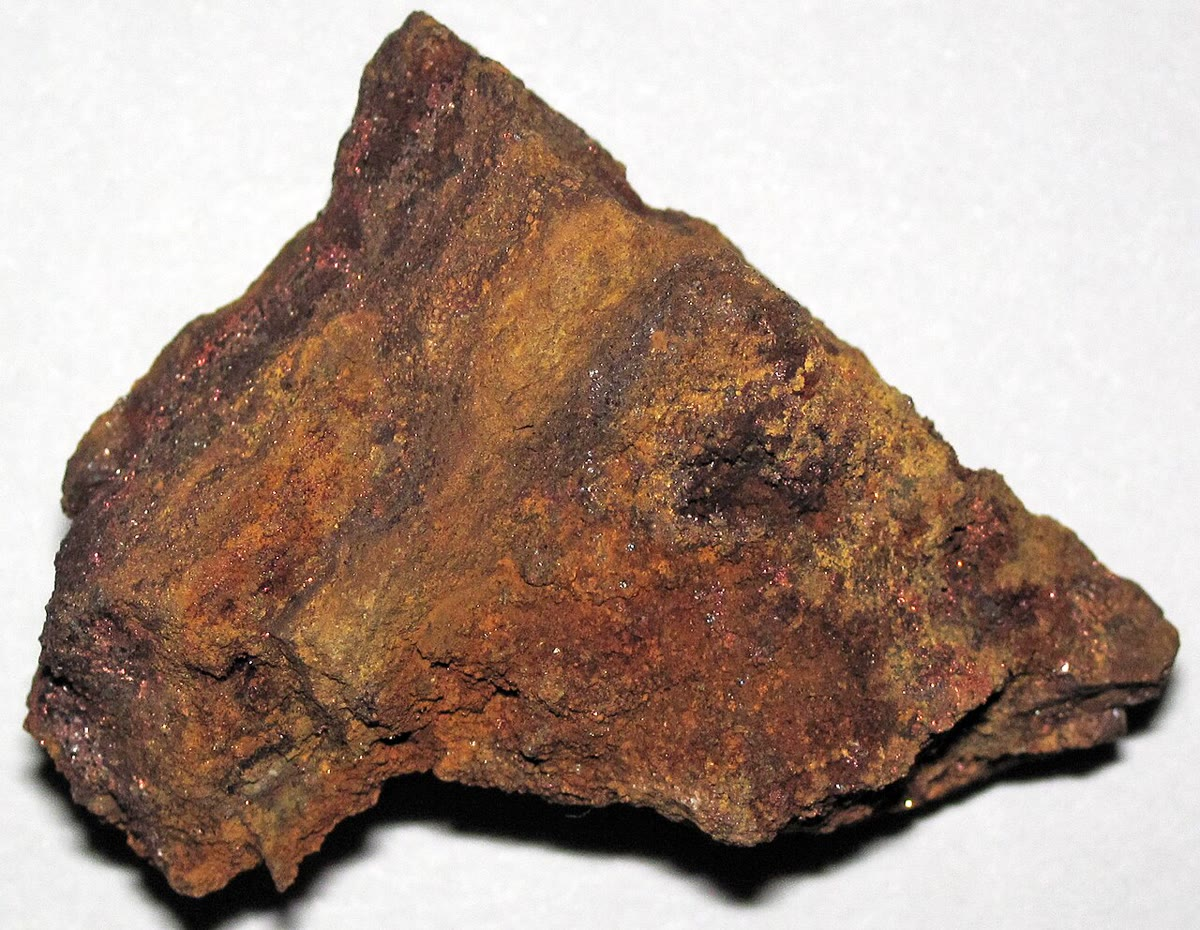
\includegraphics[width=0.4\linewidth]{images/book4/b2-29-flambeau-gossan.jpg}
\par\smallskip{\small قبّعة حديدية من مكمن فلامبو للكبريتيدات الكتلية، ويسكونسن: صخر مسامي من
هيدروكسيدات أكاسيد الحديد خلّفته تجوية البيريت والكالكوبيريت والكالكوسيت والبورنيت في
قوس بركاني من الطليعي القديم؛ والبقع البرتقالية الصغيرة نحاس طبيعي. الصورة:
\mbox{\textdir TLT James St.~John, CC BY 2.0}.}
\end{omfigure}
% ledger: photo:b2-29-gossan

\section{العيار والكتلة الطنّية}\label{sec:b2:ore-deposits:grade-tonnage}

يُدرج تجميع عالمي 422 مكمن نحاس بورفيري مع كتلتها الطنّية، عند أدنى عيار
قطع متاح، ومتوسّط عيارها من النحاس. فعُشرها يتجاوز \qty{1500}{Mt} وعُشرها يحوي أقلّ
من \qty{33}{Mt}، والوسيط \qty{240}{Mt}؛ وتمتدّ العيارات من \qty{0.24}{\percent} إلى
\qty{0.75}{\percent} بين العُشيرين نفسيهما، والوسيط \qty{0.44}{\percent}. وبين
العُشيرين تنتشر \omterm{def:b2:ore-deposits:grade}{الكتلة الطنّية} على عامل 45، والعيار على عامل 3. وعلى محاور لوغاريتمية يقترب المدرّجان كلاهما من منحنيات طبيعية، كما يبيّن الشكل أدناه:
فلوغاريتمات \omterm{def:b2:ore-deposits:grade}{الكتلة الطنّية} متوسّطها 2.373 وانحرافها المعياري 0.654، ولوغاريتمات العيار
$-0.364$ و0.199 (لوغاريتمات للأساس 10، \omterm{def:b2:ore-deposits:grade}{والكتلة الطنّية} بالميغاطنّ، والعيار بالنسبة المئوية). والملاءمة
غير تامّة: فالعيارات أشدّ تمركزًا من قانون لوغاريتمي طبيعي، وبضعة مكامن منخفضة العيار جدًا تجعلها
تحيد عنه في اختبار رسمي. والمتغيّران مستقلّان تقريبًا، بمعامل ارتباط
0.1 بين لوغاريتميهما.
% ledger: usgs08:table1, usgs08:independence, data:b4-porphyry-cu

\begin{omfigure}
\centering
\begin{minipage}[b]{0.49\linewidth}\centering
\begin{tikzpicture}
\begin{axis}[omrecord, width=0.96\linewidth, height=4.5cm, xmin=0.5, xmax=5.0, ymin=0, ymax=80,
  xlabel={الكتلة الطنّية \babelsublr{(Mt)}}, ylabel={عدد المكامن},
  xtick={1,2,3,4,5}, xticklabels={10,100,1000,$10^4$,$10^5$},
  tick label style={font=\scriptsize}, label style={font=\small}]
% computed in figdata/bachelor-2/ores.py part hist_t; ledger: data:b4-porphyry-cu
\addplot[ybar, bar width=0.22, fill=omDef!35, draw=omDef!70] table[x=log10_t, y=count] {figdata/out/bachelor-2-ores-hist_t.dat};
\addplot[omThm, line width=1pt, smooth] table[x=log10_t, y=fit] {figdata/out/bachelor-2-ores-hist_t.dat};
\end{axis}
\end{tikzpicture}
\end{minipage}\hfill
\begin{minipage}[b]{0.49\linewidth}\centering
\begin{tikzpicture}
\begin{axis}[omrecord, width=0.96\linewidth, height=4.5cm, xmin=-1.2, xmax=0.6, ymin=0, ymax=120,
  xlabel={عيار النحاس \babelsublr{(\%)}}, ylabel={عدد المكامن},
  xtick={-1,-0.69897,-0.30103,0,0.30103}, xticklabels={0.1,0.2,0.5,1,2},
  tick label style={font=\scriptsize}, label style={font=\small}]
% computed in figdata/bachelor-2/ores.py part hist_g; ledger: data:b4-porphyry-cu
\addplot[ybar, bar width=0.088, fill=omDef!35, draw=omDef!70] table[x=log10_g, y=count] {figdata/out/bachelor-2-ores-hist_g.dat};
\addplot[omThm, line width=1pt, smooth] table[x=log10_g, y=fit] {figdata/out/bachelor-2-ores-hist_g.dat};
\end{axis}
\end{tikzpicture}
\end{minipage}
\par\smallskip{\small \omterm{def:b2:ore-deposits:grade}{الكتلة الطنّية} (يمينًا) وعيار النحاس (يسارًا) لمكامن النحاس البورفيري البالغ عددها 422
في التجميع العالمي، على محاور لوغاريتمية، مع المنحنيات الطبيعية ذات المتوسّط والانحراف المعياري
نفسيهما بالأحمر. البيانات: سينغر وبيرغر ومورينغ (2008)، هيئة المسح الجيولوجي الأمريكية.}
\end{omfigure}

\begin{proposition}[جداء متغيّرات لوغاريتمية طبيعية]\label{prop:b2:ore-deposits:product}
إذا كان $\log_{10} T$ و$\log_{10} g$ طبيعيين معًا، بمتوسّطين $\mu_T$ و$\mu_g$، وانحرافين
معياريين $\sigma_T$ و$\sigma_g$ ومعامل ارتباط $\rho$، فإنّ الفلز المحتوى $M = Tg/100$
($g$ بالنسبة المئوية) لوغاريتمي طبيعي: أي إنّ $\log_{10} M$ طبيعي، حيث
\begin{equation}
\mu_M = \mu_T + \mu_g - 2 , \qquad
\sigma_M^2 = \sigma_T^2 + \sigma_g^2 + 2\rho\,\sigma_T\sigma_g .
\label{eq:b2:ore-deposits:product}
\end{equation}
\end{proposition}

\begin{proof}
$\log_{10} M = \log_{10} T + \log_{10} g - 2$. والتركيب الخطّي لمتغيّرات طبيعية معًا
طبيعي (مُسلَّم به من كتب الرياضيات)؛ ومتوسّطه مجموع المتوسّطات وتباينه
$\operatorname{var}(X + Y) = \operatorname{var} X + \operatorname{var} Y + 2\operatorname{cov}(X, Y)$،
مع $\operatorname{cov}(X, Y) = \rho\,\sigma_T\sigma_g$.
\end{proof}

وبالنسبة إلى المكامن البورفيرية، $\sigma_M = \sqrt{0.654^2 + 0.199^2 + 2 \times 0.1 \times 0.654 \times
0.199} = 0.702$ و\mbox{$\mu_M = 0.009$}: فالمكمن الوسيط يحوي نحو \qty{1}{Mt} من النحاس،
والفلز المحتوى ينتشر أوسع حتى من \omterm{def:b2:ore-deposits:grade}{الكتلة الطنّية}. والقانون اللوغاريتمي الطبيعي بهذا الانتشار الواسع
يضع معظم الفلز في مكامن قليلة: فالعُشر الأكبر يحوي نحو \qty{63}{\percent} من
النحاس وفق القانون، و\qty{64}{\percent} في البيانات (التمرين~\ref{exo:b2:ore-deposits:12}). ويرسم
الشكل أدناه كلّ مكمن بكتلته الطنّية وعياره، مع خطوط تساوي النحاس المحتوى؛
ويقع بينغهام، بمحتوى \qty{28.5}{Mt}، بين خطّي 10 و\qty{100}{Mt}.
% ledger: data:b4-porphyry-cu
% values: sd_log10_m 0.702233, mean 0.00857; median M 1.02 Mt; top 10 % share 0.631 (fit) 0.643 (data)

\begin{definition}[منحنى العيار والكتلة الطنّية]\label{def:b2:ore-deposits:gt}
\emph{منحنى العيار والكتلة الطنّية}\index{منحنى العيار والكتلة الطنّية} لمكمن يعطي، بدلالة
\omterm{def:b2:ore-deposits:grade}{عيار القطع} $c$، \omterm{def:b2:ore-deposits:grade}{الكتلة الطنّية} $T(c)$ للكتل التي يفوق عيارها $c$ ومتوسّط عيارها
$\bar g(c)$.
\end{definition}

\begin{proposition}[منحنى العيار والكتلة الطنّية لمكمن لوغاريتمي طبيعي]\label{prop:b2:ore-deposits:gt}
إذا كانت عيارات كتل مكمن كتلته الطنّية الكلّية $T_0$ لوغاريتمية طبيعية، و$\ln g$ طبيعيًّا
بمتوسّط $\mu$ (فالعيار الوسيط $e^{\mu}$) وانحراف معياري $s$، فإنّه، مع $z = (\mu -
\ln c)/s$،
\begin{equation}
T(c) = T_0\,\Phi(z), \qquad
\bar g(c) = e^{\mu + s^2/2}\,\frac{\Phi(z + s)}{\Phi(z)} ,
\label{eq:b2:ore-deposits:gt}
\end{equation}
والفلز فوق \omterm{def:b2:ore-deposits:grade}{عيار القطع} هو $M(c) = T_0\,e^{\mu + s^2/2}\,\Phi(z + s)$، أي كسر $\Phi(z +
s)$ من المجموع.
\end{proposition}

\begin{proof}
اكتب $\ln g = \mu + s u$، حيث $u$ طبيعي معياري. تكون الكتلة فوق \omterm{def:b2:ore-deposits:grade}{عيار القطع} حين $u > (\ln c -
\mu)/s = -z$، واحتمال ذلك $1 - \Phi(-z) = \Phi(z)$؛ ومنه $T(c)$. والفلز فوق
\omterm{def:b2:ore-deposits:grade}{عيار القطع} لكلّ وحدة من \omterm{def:b2:ore-deposits:grade}{الكتلة الطنّية} الكلّية هو $\int_{-z}^{\infty} e^{\mu + s u}\,\varphi(u)\,\mathrm{d}u$،
حيث $\varphi$ الكثافة الطبيعية المعيارية. وبإكمال المربّع، $e^{su}\varphi(u) =
e^{s^2/2}\varphi(u - s)$، فيكون التكامل $e^{\mu + s^2/2}\,[1 - \Phi(-z - s)] = e^{\mu +
s^2/2}\,\Phi(z + s)$. والقسمة على $\Phi(z)$ تعطي العيار المتوسّط.
\end{proof}

عندما $c \to 0$ يُحتفظ بالمكمن كلّه، بالعيار المتوسّط $e^{\mu + s^2/2}$، وهو أعلى من
الوسيط. ورفع \omterm{def:b2:ore-deposits:grade}{عيار القطع} يزيل \omterm{def:b2:ore-deposits:grade}{الكتلة الطنّية} أسرع من الفلز، لأنّ الكتل المزالة هي
الأفقر: ففي المكمن التوضيحي في الشكل، يُبقي رفع \omterm{def:b2:ore-deposits:grade}{عيار القطع} من 0.2 إلى
\qty{0.5}{\percent} على \qty{41}{\percent} من \omterm{def:b2:ore-deposits:grade}{الكتلة الطنّية} لكن على \qty{61}{\percent} من النحاس.
% values: demo T 876.0/355.0 Mt, M 4.599/2.826 Mt (figdata ores.py gtcurve)

\begin{omfigure}
\centering
\begin{minipage}[b]{0.49\linewidth}\centering
\begin{tikzpicture}
\begin{axis}[omrecord, width=0.96\linewidth, height=5.0cm, xmode=log, ymode=log,
  xmin=2, xmax=50000, ymin=0.05, ymax=2.8, xlabel={الكتلة الطنّية \babelsublr{(Mt)}}, ylabel={عيار النحاس \babelsublr{(\%)}},
  ytick={0.1,0.2,0.5,1,2}, yticklabels={0.1,0.2,0.5,1,2},
  tick label style={font=\scriptsize}, label style={font=\small}]
% computed in figdata/bachelor-2/ores.py parts scatter and iso; ledger: data:b4-porphyry-cu
\addplot[black!45, line width=0.6pt, unbounded coords=jump] table[x=tonnage_mt, y=g01] {figdata/out/bachelor-2-ores-iso.dat};
\addplot[black!45, line width=0.6pt, unbounded coords=jump] table[x=tonnage_mt, y=g1] {figdata/out/bachelor-2-ores-iso.dat};
\addplot[black!45, line width=0.6pt, unbounded coords=jump] table[x=tonnage_mt, y=g10] {figdata/out/bachelor-2-ores-iso.dat};
\addplot[black!45, line width=0.6pt, unbounded coords=jump] table[x=tonnage_mt, y=g100] {figdata/out/bachelor-2-ores-iso.dat};
\addplot[omDef, only marks, mark=*, mark size=0.8pt, opacity=0.7] table[x=tonnage_mt, y=cu_pct] {figdata/out/bachelor-2-ores-scatter.dat};
\addplot[omThm, only marks, mark=square*, mark size=2pt] coordinates {(3230,0.882)};
\node[font=\tiny, text=black!70, fill=white, inner sep=1pt] at (axis cs:4.55,2.2) {0.1};
\node[font=\tiny, text=black!70, fill=white, inner sep=1pt] at (axis cs:45.5,2.2) {1};
\node[font=\tiny, text=black!70, fill=white, inner sep=1pt] at (axis cs:455,2.2) {10};
\node[font=\tiny, text=black!70, fill=white, inner sep=1pt] at (axis cs:4545,2.2) {100 Mt};
\node[font=\scriptsize, text=omThm, anchor=south, fill=white, inner sep=1pt] at (axis cs:3230,1.0) {بينغهام};
\end{axis}
\end{tikzpicture}
\end{minipage}\hfill
\begin{minipage}[b]{0.49\linewidth}\centering
\begin{tikzpicture}
\begin{axis}[omrecord, width=0.80\linewidth, height=5.0cm, xmin=0, xmax=1.2, ymin=0, ymax=1000,
  xlabel={عيار القطع \babelsublr{(\%)}}, ylabel={الكتلة الطنّية فوق عيار القطع \babelsublr{(Mt)}}, axis y line*=left,
  ylabel style={text=omDef}, tick label style={font=\scriptsize}, label style={font=\small}]
% computed in figdata/bachelor-2/ores.py part gtcurve (illustrative deposit)
\addplot[omDef, line width=1.1pt] table[x=cutoff_pct, y=tonnage_mt] {figdata/out/bachelor-2-ores-gtcurve.dat};
\end{axis}
\begin{axis}[width=0.80\linewidth, height=5.0cm, xmin=0, xmax=1.2, ymin=0, ymax=1.6,
  axis y line*=right, axis x line=none, ylabel={العيار المتوسّط فوق عيار القطع \babelsublr{(\%)}},
  ylabel style={text=omThm}, tick label style={font=\scriptsize}, label style={font=\small}]
\addplot[omThm, line width=1.1pt, densely dashed] table[x=cutoff_pct, y=grade_pct] {figdata/out/bachelor-2-ores-gtcurve.dat};
\end{axis}
\end{tikzpicture}
\end{minipage}
\par\smallskip{\small يمينًا: \omterm{def:b2:ore-deposits:grade}{الكتلة الطنّية} وعيار النحاس لمكامن النحاس البورفيري البالغ عددها 422، مع
خطوط تساوي النحاس المحتوى (من 0.1 إلى \qty{100}{Mt})؛ والمربّع الأحمر هو بينغهام كانيون. البيانات:
سينغر وبيرغر ومورينغ (2008)، هيئة المسح الجيولوجي الأمريكية. يسارًا: \omterm{def:b2:ore-deposits:gt}{منحنى العيار والكتلة الطنّية} لمكمن توضيحي
كتلته \qty{1000}{Mt}، وعياره الوسيط \qty{0.40}{\percent}، و$s = 0.60$: \omterm{def:b2:ore-deposits:grade}{الكتلة الطنّية} فوق \omterm{def:b2:ore-deposits:grade}{عيار القطع} (بالأزرق)
وعيارها المتوسّط (بالأحمر، متقطّعًا)، من \eqref{eq:b2:ore-deposits:gt}.}
\end{omfigure}

\section{التنقيب}\label{sec:b2:ore-deposits:exploration}

تُكتشف المكامن بالآثار التي تتركها خارج خامها. فهالة التبدّل في نظام بورفيري
عرضها كيلومترات، وحيث يتكشّف الصخر يمكن رسم خرائط معادنها من الطائرات
والأقمار الصناعية بأطيافها تحت الحمراء؛ وتتشتّت فلزّاته في الترب ورواسب المجاري والمياه والنباتات المحيطة
به؛ وتغيّر كبريتيداته وصخوره المتبدّلة الخواصّ الفيزيائية التي تقيسها الجيوفيزياء.
% ledger: usgs10b:form, usgs10b:exploration, usgs10b:remote

\begin{definition}[الشذوذ الجيوكيميائي]\label{def:b2:ore-deposits:exploration}
\emph{الشذوذ الجيوكيميائي}\index{الشذوذ الجيوكيميائي} تركيز لعنصر، أو لمجموعة من
العناصر، في وسط تؤخذ منه العيّنات --- صخر، وتربة، ورواسب مجارٍ، وماء، ونباتات --- يحيد
عن خلفيته في المنطقة، أي مدى التركيزات الموجود حيث لا يوجد
تمعدن.
\end{definition}

وكالعيارات، تنتشر التركيزات على عدّة مراتب عشرية، ولذا يُحكم على الشذوذ عادة بدلالة
اللوغاريتمات؛ ومن العتبات البسيطة، المستعملة في التمرين~\ref{exo:b2:ore-deposits:9}، متوسّط
لوغاريتمات الخلفية مضافًا إليه ضعف انحرافها المعياري. وعيّنة رواسب المجرى
تخلط رواسب حوضها كلّه، فيخبو الشذوذ مع اتجاه التيار كلّما انضمّت إليها رواسب نظيفة،
ويشير تدرّج التركيزات إلى أعلى شبكة التصريف نحو المصدر. وفي الترب فوق
بيغماتيتات مدفونة، تُتُبّعت شذوذات الليثيوم والروبيديوم والسيزيوم والتنتالوم والقصدير فوق
أجسام لا تتكشّف.
% ledger: usgs10b:exploration, usgs10o:lct

وتُختار الطرائق الجيوفيزيائية بحسب التباين الذي يقدّمه نمط المكمن. فالكبريتيدات المنتشرة تجعل
الصخر يتصرّف كالمكثّف: وطريقة الاستقطاب المستحثّ، التي تقيس هذه القابلية للشحن، طُوّرت
للنحاس البورفيري وتستجيب أكثر ما تستجيب للنطاق السيريسيتي الغني بالبيريت، إذ إنّ اللبّ البوتاسي
أفقر بالكبريتيدات. وترسم المسوح المغناطيسية والجاذبية خرائط البلوتونات التي ترتبط بها المكامن.
ولا طريقة ترى الخام
مباشرة، وكلّ تفسير غير وحيد حتى يختبره ثقب حفر.
% ledger: usgs10b:exploration

\begin{method}[من التحاليل إلى تقدير المورد]\label{met:b2:ore-deposits:resource}
البيانات ثقوب حفر على شبكة عبر المكمن، يُوصف لبابها ويُحلَّل على فترات
معلومة الطول.
\begin{enumerate}
  \item \textbf{التركيب.} احسب متوسّط التحاليل على أطوال متساوية، مرجِّحًا كلّ تحليل
        بطوله، بحيث تمثّل كلّ عيّنة مركّبة الحجم نفسه.
  \item \textbf{النموذج.} قسّم المكمن إلى كتل وقدّر عيار كلّ منها من
        العيّنات المركّبة القريبة، مرجِّحًا إيّاها بالمسافة وبالارتباط المكاني للعيارات
        (طريقة الكريغينغ الجيوإحصائية، مُسلَّم بها).
  \item \textbf{التقرير.} طبّق عيار قطع: \omterm{def:b2:ore-deposits:grade}{الكتلة الطنّية} والعيار المتوسّط للكتل التي تفوقه، مع
        كثافة الصخر، عند كلّ مستوى ثقة يسمح به تباعد ثقوب الحفر.
\end{enumerate}
\end{method}

\begin{inthefield}[وصف لباب الحفر]
\centering
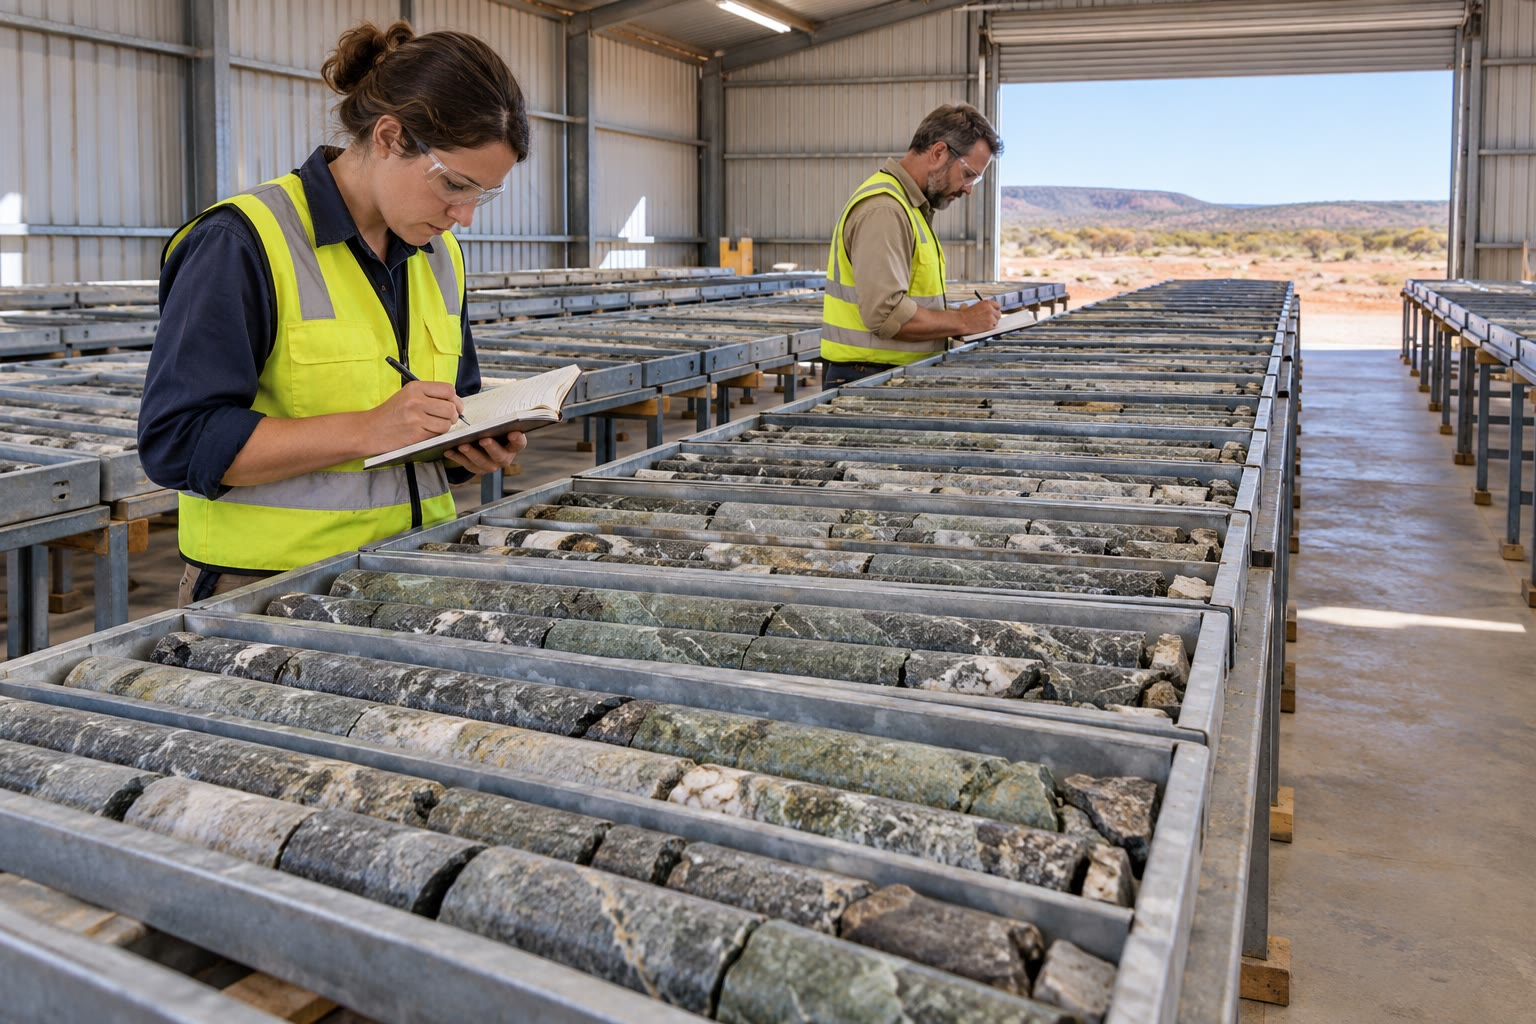
\includegraphics[width=0.56\linewidth]{images/book4/ai/b2-core-shed.jpg}
\par\smallskip{\small مستودع للباب الحفر في مشروع تنقيب (رسم توضيحي مولَّد بالذكاء الاصطناعي).}
\par\medskip\raggedright
في مشروع التنقيب، يُصفّ اللباب المستخرج من كلّ ثقب حفر في صناديق معدنية بالترتيب الذي
خرج به من الأرض. ويمشي الجيولوجيون على طول الصناديق، فترة بعد فترة، ويسجّلون ماهيّة
الصخر، وكيف تبدّل، وأيّ العروق تقطعه وبأيّ نسبة، وأيّ الكبريتيدات
يحوي؛ ويعلّمون المواضع التي سيُنشر فيها اللباب وتؤخذ منه العيّنات. ويأتي الوصف قبل التحاليل ويُقارن
بها: فنطاق التبدّل أو نمط العروق الذي يحمل الفلز يصبح الشيء الذي
يُتتبّع من ثقب إلى ثقب، ومن الوصف يرسم الجيولوجيون المقاطع التي تُخطَّط منها الثقوب
التالية.
\end{inthefield}

\section*{التمارين}\label{sec:b2:ore-deposits:exercises}

معطيات التمارين، ما لم يُذكر غير ذلك: القشرة القارّية العليا، النحاس \qty{28}{ppm}،
والذهب \qty{1.5}{ng/g}، والكروم \qty{92}{ppm}؛ ومجتمع النحاس البورفيري في
\cref{sec:b2:ore-deposits:grade-tonnage}، $\log_{10}$ \omterm{def:b2:ore-deposits:grade}{الكتلة الطنّية} (بالميغاطنّ) متوسّطه 2.373 وانحرافه
المعياري 0.654، و$\log_{10}$ العيار (بالنسبة المئوية) متوسّطه $-0.364$ وانحرافه المعياري 0.199، ومعامل الارتباط
$\rho = 0.100$. قرّب إلى ثلاثة أرقام معنوية.
% ledger: rg03:ucc-trace, data:b4-porphyry-cu

\begin{exercise}[$\star$]\label{exo:b2:ore-deposits:1}
أوجد \omterm{def:b2:ore-deposits:cf}{معامل التركيز} مقارنة بالقشرة العليا لكلّ من: (أ) خام نحاس عياره
\qty{0.5}{\percent}؛ (ب) خام ذهب عياره \qty{6}{g/t}؛ (ج) كروميتيت يحوي \qty{90}{\percent}
من الكروميت، باعتبار الكروميت \babelsublr{FeCr$_2$O$_4$} (الكتل الذرية: الكروم 52.00، والحديد 55.85، والأكسجين 16.00).
\end{exercise}

\begin{exercise}[$\star$]\label{exo:b2:ore-deposits:2}
يُعلَن مكمن باتو هيجاو بكتلة \qty{914}{Mt} وعيار \qty{0.53}{\percent} من النحاس و\qty{0.40}{g/t} من الذهب فوق
عيار قطع \qty{0.3}{\percent}، وبكتلة \qty{1640}{Mt} وعيار \qty{0.44}{\percent} من النحاس و\qty{0.45}{g/t}
من الذهب عند أدنى عيار قطع متاح. (أ) أوجد النحاس المحتوى (بالميغاطنّ) والذهب (بالطنّ) في كلّ
تقدير. (ب) ما \omterm{def:b2:ore-deposits:grade}{الكتلة الطنّية} وما النحاس اللذان تضيفهما الكتل الإضافية في التقدير الثاني، وبأيّ
عيار متوسّط؟ (ج) لماذا كلا التقديرين صحيح؟
\end{exercise}

\begin{exercise}[$\star$]\label{exo:b2:ore-deposits:3}
في قانون ستوكس تتناسب سرعة ترسّب حبيبة قطرها $d$ مع $(\rho_s -
\rho_w)\,d^2$. خذ $\rho_w = 1.00$، والكوارتز 2.65، والذهب 19.3، والزركون 4.7 (بوحدة
\unit{g.cm^{-3}}). (أ) كم مرّة تترسّب حبيبة ذهب أسرع من حبيبة كوارتز لها
الحجم نفسه؟ (ب) ما نسبة قطري حبيبة ذهب وحبيبة كوارتز تترسّبان
بالسرعة نفسها؟ (ج) أيّ حبيبة كوارتز تترسّب كحبيبة زركون قطرها \qty{0.1}{mm}؟
\end{exercise}

\begin{exercise}[$\star$]\label{exo:b2:ore-deposits:4}
خام نحاس أوّلي عياره \qty{0.4}{\percent}. تغسل التجوية كلّ نحاسه على
سمك \qty{150}{m} وتعيد ترسيبه في غطاء سمكه \qty{50}{m} تحته مباشرة، مع بقاء الكثافة
نفسها. (أ) أوجد عيار الغطاء. (ب) الأمر نفسه إذا لم يُعَد ترسيب إلا \qty{80}{\percent} من
النحاس المغسول. (ج) أيّ سمك مغسول يعطي \qty{1.7}{\percent} مع إعادة
ترسيب كاملة؟
\end{exercise}

\begin{exercise}[$\star\star$]\label{exo:b2:ore-deposits:5}
تحوي صهارة \qty{10}{ppb} من البلاتين و\qty{200}{ppm} من النيكل؛ خذ $D_{\mathrm{Pt}} =
10^4$ و$D_{\mathrm{Ni}} = 500$. (أ) باستعمال \eqref{eq:b2:ore-deposits:r-factor}، أوجد
محتوى الكبريتيد من البلاتين (بوحدة ppm) والنيكل (بالنسبة المئوية الوزنية) عندما $R = 100$ و\num{1000} و\num{10000}
و\num{100000}. (ب) أوجد نهايتيهما عندما $R \to \infty$. (ج) اشرح لماذا لا يقول خام النيكل
إلا القليل عن $R$، بينما يقول خام البلاتين الكثير.
\end{exercise}

\begin{exercise}[$\star\star$]\label{exo:b2:ore-deposits:6}
باستعمال \eqref{eq:b2:ore-deposits:product} لمجتمع النحاس البورفيري: (أ) أوجد متوسّط
$\log_{10} M$ وانحرافه المعياري، والنحاس المحتوى الوسيط. (ب) ما كسر المكامن
الذي يحوي أكثر من \qty{10}{Mt} من النحاس؟ وكم مكمنًا من 422؟ (ج) أعد (ب) مع إهمال الارتباط.
\end{exercise}

\begin{exercise}[$\star\star$]\label{exo:b2:ore-deposits:7}
للمكمن التوضيحي في الشكل ($T_0 = \qty{1000}{Mt}$، والوسيط \qty{0.40}{\percent}،
$s = 0.60$)، استعمل \eqref{eq:b2:ore-deposits:gt} لإيجاد \omterm{def:b2:ore-deposits:grade}{الكتلة الطنّية} والعيار المتوسّط والنحاس المحتوى
فوق عياري قطع \qty{0.3}{\percent} و\qty{0.6}{\percent}. تحقّق من نقطة واحدة على الشكل.
\end{exercise}

\begin{exercise}[$\star\star$]\label{exo:b2:ore-deposits:8}
مكمن بورفيري يحوي \qty{5}{Mt} من النحاس. افترض أنّ مائعه الصهاري حمل \qty{1000}{ppm}
من النحاس، ترسّب نصفها في الخام، وأنّ \omterm{def:b2:magma-emplacement:magma}{الصهارة} أطلقت \qty{3.5}{\percent}
من كتلتها مائعًا. (أ) أوجد كتلة المائع وكتلة \omterm{def:b2:magma-emplacement:magma}{الصهارة} اللازمتين. (ب) أوجد حجم
\omterm{def:b2:magma-emplacement:magma}{الصهارة}، وكثافتها \qty{2600}{kg.m^{-3}}. (ج) إذا كانت \omterm{def:b2:magma-emplacement:magma}{الصهارة} تحوي \qty{50}{ppm} من النحاس، فما الكسر
الذي انتهى منه في الخام؟
\end{exercise}

\begin{exercise}[$\star\star$]\label{exo:b2:ore-deposits:9}
تعطي ثماني عيّنات من رواسب مجارٍ في الخلفية القيم التالية للمقدار \babelsublr{$\log_{10}$ Cu (ppm)}: 1.30، 1.45، 1.38، 1.52، 1.41، 1.35،
1.48 و1.40. (أ) أوجد متوسّط اللوغاريتمات وانحرافها المعياري (للمجتمع)، ووسيط
الخلفية والعتبة، أي المتوسّط مضافًا إليه ضعف الانحراف المعياري، بوحدة ppm. (ب) رافد
يصرّف \qty{4}{km^2} من أرض متمعدنة يحمل رواسب بتركيز \qty{400}{ppm}؛ وينضمّ إلى مجرى
يصرّف \qty{36}{km^2} عند وسيط الخلفية. بافتراض أنّ كلّ كيلومتر مربّع يعطي الكتلة نفسها
من الرواسب، هل الرواسب المختلطة شاذّة؟ (ج) إلى أيّ مساحة حوض كلّية يبقى
الشذوذ فوق العتبة؟
\end{exercise}

\begin{exercise}[$\star\star\star$]\label{exo:b2:ore-deposits:10}
(أ) أثبت أنّ $e^{su}\varphi(u) = e^{s^2/2}\varphi(u - s)$. (ب) استنتج متوسّط متغيّر لوغاريتمي
طبيعي، $e^{\mu + s^2/2}$. (ج) بيّن أنّ كسر الفلز فوق \omterm{def:b2:ore-deposits:grade}{عيار القطع}،
$\Phi(z + s)$، يفوق دائمًا كسر \omterm{def:b2:ore-deposits:grade}{الكتلة الطنّية}، $\Phi(z)$، وفسّر ذلك.
\end{exercise}

\begin{exercise}[$\star\star\star$]\label{exo:b2:ore-deposits:11}
(أ) انطلاقًا من \eqref{eq:b2:ore-deposits:r-factor}، أوجد قيمة $R$ التي يبلغ عندها $C_S$ كسرًا $f$
من سقفه $D\,C_L$. (ب) احسبها عندما $f = 0.5$ و$0.9$ مع $D = 300$ (النيكل) و$D =
10^4$ (البلاتين). (ج) قارن بمديات $R$ لخامات النيكل والنحاس ولحيود عناصر مجموعة البلاتين المذكورة
في النصّ.
\end{exercise}

\begin{exercise}[$\star\star\star$]\label{exo:b2:ore-deposits:12}
(أ) لمتغيّر لوغاريتمي طبيعي $M$ يكون فيه الانحراف المعياري للمقدار $\ln M$ مساويًا $s$، بيّن أنّ المكامن التي تقع
فوق الكمّية ذات الرتبة $q$ تحوي كسرًا $\Phi\bigl(s - \Phi^{-1}(q)\bigr)$ من الفلز الكلّي.
(ب) احسبه لمجتمع النحاس البورفيري و$q = 0.9$. (ج) الأمر نفسه عندما $q = 0.99$؛ وقارن
بالمكامن الأربعة الكبرى، التي تحوي \qty{26.6}{\percent} من نحاس التجميع.
\end{exercise}
% ledger: data:b4-porphyry-cu

\begin{problem}[{مسألة نهاية الأسبوع --- موقع تنقيب بورفيري واعد}]\label{pb:b2:ore-deposits:1}
حُفر موقع تنقيب بورفيري واعد (مُتخيَّل). وقد قطع ثقب الاكتشاف فيه ثماني فترات، من الأعلى
إلى الأسفل (الطول بالأمتار، وعيار النحاس بالنسبة المئوية): 30 مترًا بعيار 0.12؛ و40 بعيار 0.35؛ و50 بعيار 0.62؛ و60
بعيار 0.48؛ و40 بعيار 0.27؛ و30 بعيار 0.81؛ و50 بعيار 0.41؛ و30 بعيار 0.18. وتجد دراسة جيوإحصائية لكلّ الثقوب
أنّ عيارات الكتل لوغاريتمية طبيعية، بوسيط \qty{0.38}{\percent} و$s = 0.55$ للمقدار
$\ln g$. والجسم المتمعدن قريب من أسطوانة رأسية نصف قطرها \qty{450}{m} وارتفاعها
\qty{700}{m}، وكثافتها \qty{2.7}{t.m^{-3}}. استعمل معطيات التمارين، وقرّب إلى ثلاثة
أرقام معنوية (والاحتمالات إلى أربعة).

\noindent\textbf{الجزء الأول --- ثقب الاكتشاف.}
\begin{enumerate}
  \item أوجد طول الثقب المأخوذة منه العيّنات وعياره المتوسّط المرجَّح بالطول.
  \item أوجد المتوسّط الحسابي للعيارات الثمانية. لماذا يكون المتوسّط المرجَّح هو الصحيح؟
  \item ما كسر الطول الذي يفوق عياره \qty{0.3}{\percent}، وبأيّ عيار متوسّط؟
  \item أوجد \omterm{def:b2:ore-deposits:cf}{معامل التركيز} للعيار المتوسّط المرجَّح مقارنة بالقشرة العليا.
  \item الأمر نفسه لأغنى فترة.
  \item أوجد العيار المتوسّط لكلّ كتل المكمن. هل ثقب الاكتشاف ممثِّل؟
\end{enumerate}

\noindent\textbf{الجزء الثاني --- \omterm{def:b2:ore-deposits:grade}{الكتلة الطنّية} فوق \omterm{def:b2:ore-deposits:grade}{عيار القطع}.}
\begin{enumerate}[resume]
  \item أوجد حجم الجسم وكتلته الطنّية $T_0$؛ واحتفظ بالقيمة $T_0 = \qty{1200}{Mt}$.
  \item لعيار قطع \qty{0.3}{\percent}، أوجد $z$ وكسر الكتل التي تفوقه.
  \item أوجد \omterm{def:b2:ore-deposits:grade}{الكتلة الطنّية} فوق عيارات قطع 0.2 و0.3 و\qty{0.5}{\percent}.
  \item أوجد العيار المتوسّط فوق \omterm{def:b2:ore-deposits:grade}{عيار القطع} \qty{0.3}{\percent}.
  \item الأمر نفسه فوق 0.2 و\qty{0.5}{\percent}.
  \item عند رفع \omterm{def:b2:ore-deposits:grade}{عيار القطع} من 0.3 إلى \qty{0.5}{\percent}: بأيّ عاملين تتغيّر \omterm{def:b2:ore-deposits:grade}{الكتلة الطنّية}
        والعيار المتوسّط؟
  \item عند أيّ عيار قطع يُحتفظ بنصف \omterm{def:b2:ore-deposits:grade}{الكتلة الطنّية}، وما عيارها المتوسّط؟
\end{enumerate}

\noindent\textbf{الجزء الثالث --- الموقع الواعد بين بورفيريات العالم.}
\begin{enumerate}[resume]
  \item أوجد النحاس المحتوى في الجسم كلّه، بعياره المتوسّط.
  \item أوجد الدرجة المعيارية لكتلته الطنّية في المجتمع العالمي، ومئينها.
  \item الأمر نفسه لعياره المتوسّط.
  \item أوجد الانحراف المعياري للمقدار $\log_{10} M$ مع الارتباط، ومن دونه.
  \item أوجد مئين النحاس المحتوى فيه.
  \item كم مكمنًا من المكامن البالغ عددها 422 يُتوقّع أن يحوي نحاسًا أكثر منه؟
\end{enumerate}

\noindent\textbf{الجزء الرابع --- النحاس فوق \omterm{def:b2:ore-deposits:grade}{عيار القطع}.}
\begin{enumerate}[resume]
  \item أوجد النحاس المحتوى فوق \omterm{def:b2:ore-deposits:grade}{عيار القطع} \qty{0.2}{\percent}.
  \item الأمر نفسه فوق \qty{0.5}{\percent}.
  \item ما كسر النحاس الذي يقع فوق \qty{0.3}{\percent}، وما كسر
        \omterm{def:b2:ore-deposits:grade}{الكتلة الطنّية}؟
  \item اشرح لماذا يضيف خفض \omterm{def:b2:ore-deposits:grade}{عيار القطع} إلى ما دون \qty{0.3}{\percent} صخرًا كثيرًا ونحاسًا
        قليلًا، مستعينًا بجوابي السؤالين 9 و20.
  \item خلاصة القول: كم من النحاس يحوي الموقع الواعد فوق \omterm{def:b2:ore-deposits:grade}{عيار القطع} \qty{0.3}{\percent}؟
\end{enumerate}
\end{problem}
